% Lecture Template for ME3001-001-Tristan Hill - Spring 2017
% 
% Mechanical Engineering Analysis with MATLAB
%
% SOridnary Differential Equations - Lecture 1


% Document settings
\documentclass[11pt]{article}
\usepackage[margin=1in]{geometry}
\usepackage[pdftex]{graphicx}
\usepackage{multirow}
\usepackage{setspace}
\usepackage{hyperref}
\usepackage{color,soul}
\usepackage{fancyvrb}
\usepackage{framed}
\usepackage{wasysym}
\usepackage{multicol}

\pagestyle{plain}
\setlength\parindent{0pt}
\hypersetup{
    bookmarks=true,         % show bookmarks bar?
    unicode=false,          % non-Latin characters in Acrobat’s bookmarks
    pdftoolbar=true,        % show Acrobat’s toolbar?
    pdfmenubar=true,        % show Acrobat’s menu?
    pdffitwindow=false,     % window fit to page when opened
    pdfstartview={FitH},    % fits the width of the page to the window
    pdftitle={My title},    % title
    pdfauthor={Author},     % author
    pdfsubject={Subject},   % subject of the document
    pdfcreator={Creator},   % creator of the document
    pdfproducer={Producer}, % producer of the document
    pdfkeywords={keyword1} {key2} {key3}, % list of keywords
    pdfnewwindow=true,      % links in new window
    colorlinks=true,       % false: boxed links; true: colored links
    linkcolor=red,          % color of internal links (change box color with linkbordercolor)
    citecolor=green,        % color of links to bibliography
    filecolor=magenta,      % color of file links
    urlcolor=blue           % color of external links
}

% assignment number 
\newcommand{\NUM}{1} 
\newcommand{\VSpaceSize}{2mm} 
\newcommand{\HSpaceSize}{2mm} 
\newcommand{\VSPC}{15mm} 


\definecolor{mygray}{rgb}{.6, .6, .6}
% [153,50,204] - dark orchid
\definecolor{mypurple}{rgb}{0.6,0.1961,0.8}
%[139,69,19] - saddle brown
\definecolor{mybrown}{rgb}{0.5451,0.2706,0.0745}
\setulcolor{red} 
\setstcolor{green} 
\sethlcolor{mygray} 

\begin{document}

\textbf{ \LARGE ME 3001 Lecture, Ordinary Differential Equations} \\\\
\textbf{ \LARGE A Brief Review of to Begin} \\

\begin{itemize}

	\item  \textbf{\LARGE What is a Differential Equation?}
		\LARGE
		\begin{itemize}
			\item An equation describing a function and one or more of its derivatives of the \color{mypurple}dependent variable \color{black} with respect to the \\ \color{blue} independent variable\color{black}. \\ \vspace{10mm}
			
			\item \color{mypurple}Dependent Variable \color{black}	\\\vspace{20mm}
			
			\item \color{blue} Independent Variable\color{black} \\\vspace{20mm}
		\end{itemize}	

	\item \textbf{\LARGE Standard form of a O.D.E.} \vspace{10mm}\\
			\scalebox{1.2}{$a_n\frac{dy^{(n)}}{d^{(n)}x}+a_{n-1}\frac{dy^{(n-1)}}{d^{(n-1)}x}+...+a_{2}\frac{dy^{2}}{d^{2}x}+a_{1}\frac{dy}{dx}+a_0=f(x)$}	\vspace{10mm}\\		
			\scalebox{1.2}{$a_ny^{(n)}+a_{n-1}y^{(n-1)}+...+a_2y'' +a_1y'+a_0=f(x)$}

\newpage
\item \textbf{\LARGE Classification of Ordinary Differential Equations} \\
	\begin{itemize}
		\item Ordinary or Partial\vspace{\VSPC} \\
		\item Homogeneous or In-Homogeneous\vspace{\VSPC} \\
		\item Order of the Equation\vspace{\VSPC} \\
		\item Linear or Non-Linear \vspace{\VSPC} 
		\begin{itemize}
			\item 1)\\
			\item 2)\vspace{\VSPC} \\
		\end{itemize}
		\item Degree of the Equation\\ \\
		
	\end{itemize}

\newpage
\item \textbf{\LARGE Classification Examples}


\newpage
\item \textbf{\LARGE Differential Equations in Engineering}

	\begin{itemize}

		\item \textbf{ \LARGE The Study of how physical quantities vary with respect to each other in space and time.}\\
		\item Dynamics \\
		\item Heat Transfer\\
		\item Vibrations\\
		\item Possibly the Most Common ODE in Engineering...\\
	
		
			

	\end{itemize}


\newpage

\item \textbf{\LARGE A Mechanical Engineering Example}\\\\	


		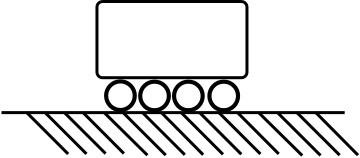
\includegraphics[scale=0.75]{lecture1_fig3.png}\\
		
		
\newpage

\item \textbf{\LARGE Derivation of the O.D.E.}\\\\	
		
\newpage

\item \textbf{\LARGE Solution of the O.D.E.}\\\\	
		
\newpage

\item \textbf{\LARGE What does it look like?}

	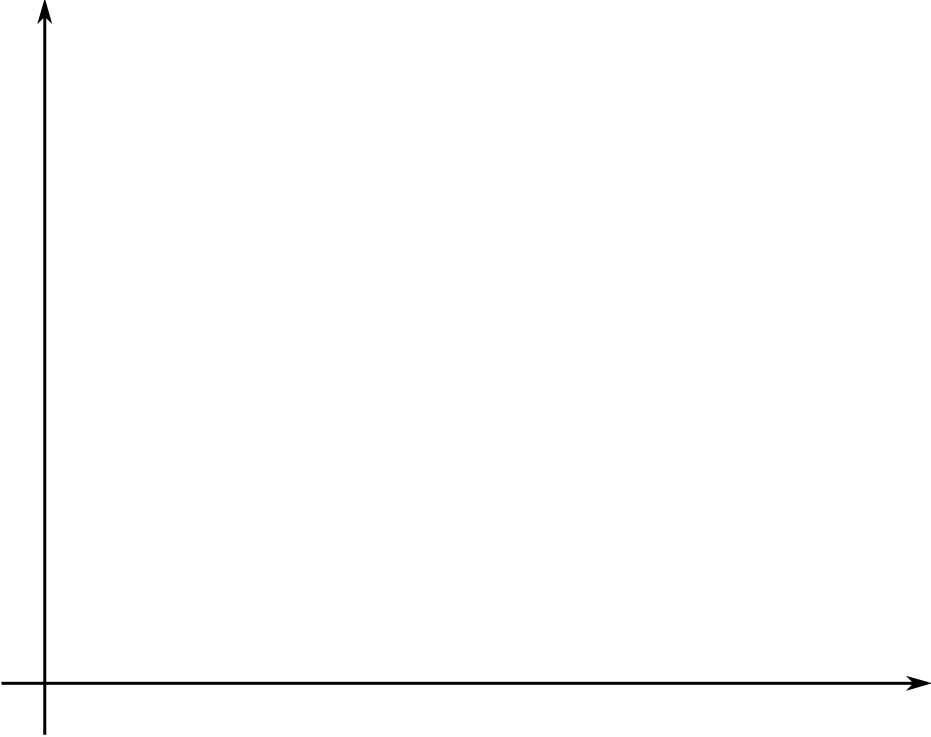
\includegraphics[scale=0.4]{lecture1_fig2.png}\\
	
	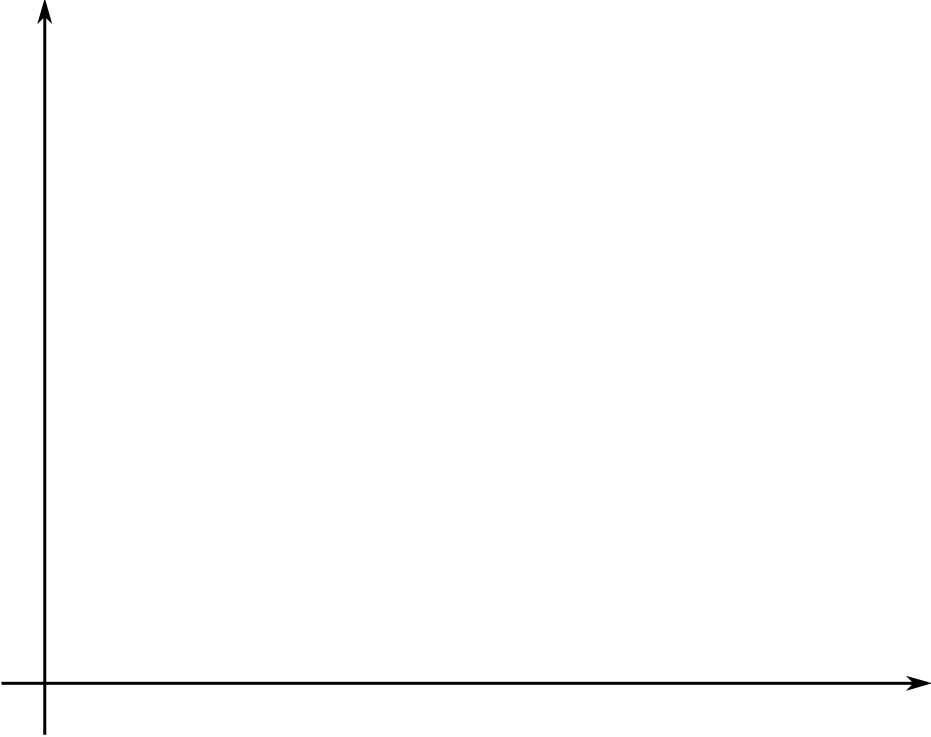
\includegraphics[scale=0.4]{lecture1_fig2.png}\\	


\end{itemize}


	

\end{document}



